%==============================================================================
% Sjabloon poster bachproef
%==============================================================================
% Gebaseerd op document class `a0poster' door Gerlinde Kettl en Matthias Weiser
% Aangepast voor gebruik aan HOGENT door Jens Buysse en Bert Van Vreckem

\documentclass[a0,portrait]{hogent-poster}

% Info over de opleiding
\course{Bachelorproef}
\studyprogramme{toegepaste informatica}
\academicyear{2024-2025}
\institution{Hogeschool Gent, Valentin Vaerwyckweg 1, 9000 Gent}

% Info over de bachelorproef
\title{De praktische voordelen van RESTful API design in een Laravel-API}
\subtitle{Een case study bij BrightAnalytics}
\author{Lars Salembier}
\email{lars.salembier@student.hogent.be}
\supervisor{Irina Malfait}
\cosupervisor{Lowie Tyvaert (BrightAnalytics)}

% Indien ingevuld, wordt deze informatie toegevoegd aan het einde van de
% abstract. Zet in commentaar als je dit niet wilt.
\specialisation{Web en Enterprise Development}
\keywords{RESTful API, OpenAPI, Laravel, API Design}
\projectrepo{https://github.com/larssalembier/bachelorproef}

\begin{document}

\maketitle

\begin{abstract}
In de hedendaagse, sterk verbonden digitale wereld zijn Application Programming Interfaces (API's) de onmisbare bouwstenen voor interactie tussen applicaties en systemen. Voor BrightAnalytics, een bedrijf dat een geavanceerd data-visualisatieplatform voor financiële rapportage en business intelligence maakt, is de kwaliteit, robuustheid en schaalbaarheid van hun API's van cruciaal belang voor het succes van hun product. Deze bachelorproef duikt diep in de wereld van RESTful API design, inclusief de principes van HATEOAS (Hypermedia as the Engine of Application State) en OpenAPI, om te onderzoeken hoe deze concepten kunnen bijdragen aan de optimalisatie van API-ontwikkeling binnen BrightAnalytics, met specifieke focus op hoe we deze principes kunnen toepassen bij de ontwikkeling van een API met Laravel. De centrale onderzoeksvraag is: ``Welke concrete voordelen biedt de implementatie van RESTful API design, en in het bijzonder HATEOAS en OpenAPI, voor de kwaliteit, consistentie en onderhoudbaarheid van een Laravel-API en een bijbehorende frontend applicatie?''. Door middel van een grondige literatuurstudie en een praktische case study, de ontwikkeling van de BrightEats API – een intern platform voor lunchbestellingen – worden deze principes geëvalueerd op hun impact op backend- en frontend-ontwikkeling, ontwikkelingskosten, onderhoudbaarheid, en de algehele UX (user experience) en DX (developer experience).
\end{abstract}

\begin{multicols}{2} % This is how many columns your poster will be broken into, a portrait poster is generally split into 2 columns

\section{Inleiding}

Deze bachelorproef onderzoekt hoe RESTful API design, HATEOAS en OpenAPI kunnen bijdragen aan het optimaliseren van API-ontwikkeling binnen BrightAnalytics, met specifieke aandacht voor de implementatie in Laravel. De BrightEats applicatie, een intern platform voor lunchbestellingen, dient als een concrete case study om de praktische implementatie en evaluatie van deze principes te illustreren.

\section{Literatuurstudie: diepgaande analyse van REST, HATEOAS en OpenAPI}

De literatuurstudie vormt de theoretische basis van dit onderzoek en omvat een diepgaande analyse van RESTful API design principes, HATEOAS en OpenAPI. REST, Representational State Transfer, beschrijft een API als een uniforme interface voor interactie met resources, die worden geïdentificeerd via URI's en gemanipuleerd via standaard HTTP-methoden (GET, POST, PUT, DELETE, PATCH). HATEOAS, Hypermedia as the Engine of Application State, introduceert het concept van hypermedialinks in API-responses, waardoor clients dynamisch kunnen navigeren door de API zonder voorafgaande kennis van de URI-structuur. OpenAPI, voorheen Swagger, biedt een gestandaardiseerde manier om API's te beschrijven en te documenteren, wat de samenwerking tussen ontwikkelaars en de integratie met andere systemen vergemakkelijkt.

\section{Opgestelde RESTful API Guidelines}

Gebaseerd op de inzichten uit de literatuurstudie en de specifieke context van BrightAnalytics, werden concrete guidelines opgesteld voor de ontwikkeling van RESTful API's, gebaseerd op de Zalando RESTful API Guidelines. Deze guidelines behandelen diverse aspecten van API design, waaronder URI-structuur, HTTP-methoden, statuscodes, dataformaten, error handling, versiebeheer en authenticatie.

\section{Case Study: BrightEats API}

De BrightEats API, een intern platform ontwikkeld voor het beheren van lunchbestellingen binnen BrightAnalytics, diende als een praktische case study voor dit onderzoek. De API biedt functionaliteit voor het beheren van gebruikers, winkels, menu's, groepsbestellingen en betalingen, inclusief de generatie van QR-codes voor mobiele betalingen. De implementatie van de API volgde een iteratieve aanpak, waarbij stapsgewijs functionaliteit werd toegevoegd en verfijnd op basis van de opgestelde guidelines.

\section{Implementatie met Laravel}

De backend van de BrightEats API werd ontwikkeld met alle guidelines in het achterhoofd. Resource controllers bieden een gestructureerde manier om CRUD-operaties (Create, Read, Update, Delete) op resources te implementeren. Policies worden gebruikt voor autorisatie, waardoor gecontroleerd kan worden welke gebruikers toegang hebben tot specifieke resources en acties. Request classes zorgen voor validatie van inkomende data, terwijl services, zoals de \texttt{OrderService} en \texttt{QrCodeGenerator}, de business logica encapsuleren. API Resources transformeren de data naar een formaat dat geschikt is voor consumptie door de frontend.

\section{OpenAPI}

De OpenAPI-specificatie speelt een cruciale rol in de documentatie en standaardisatie van de BrightEats API. De specificatie wordt gegenereerd met behulp van de \texttt{dedoc/scramble}-package, die PHPDoc comments in de code gebruikt om een OpenAPI-document te creëren. Deze automatisch gegenereerde documentatie dient als een centrale bron van waarheid voor alle ontwikkelaars die met de API werken, zowel frontend als backend. De interactieve documentatie, automatisch gegenereerd vanuit de OpenAPI-specificatie, vergemakkelijkt de samenwerking tussen teams en versnelt het onboarding proces voor nieuwe ontwikkelaars.

\begin{center}
  \captionsetup{type=figure}
  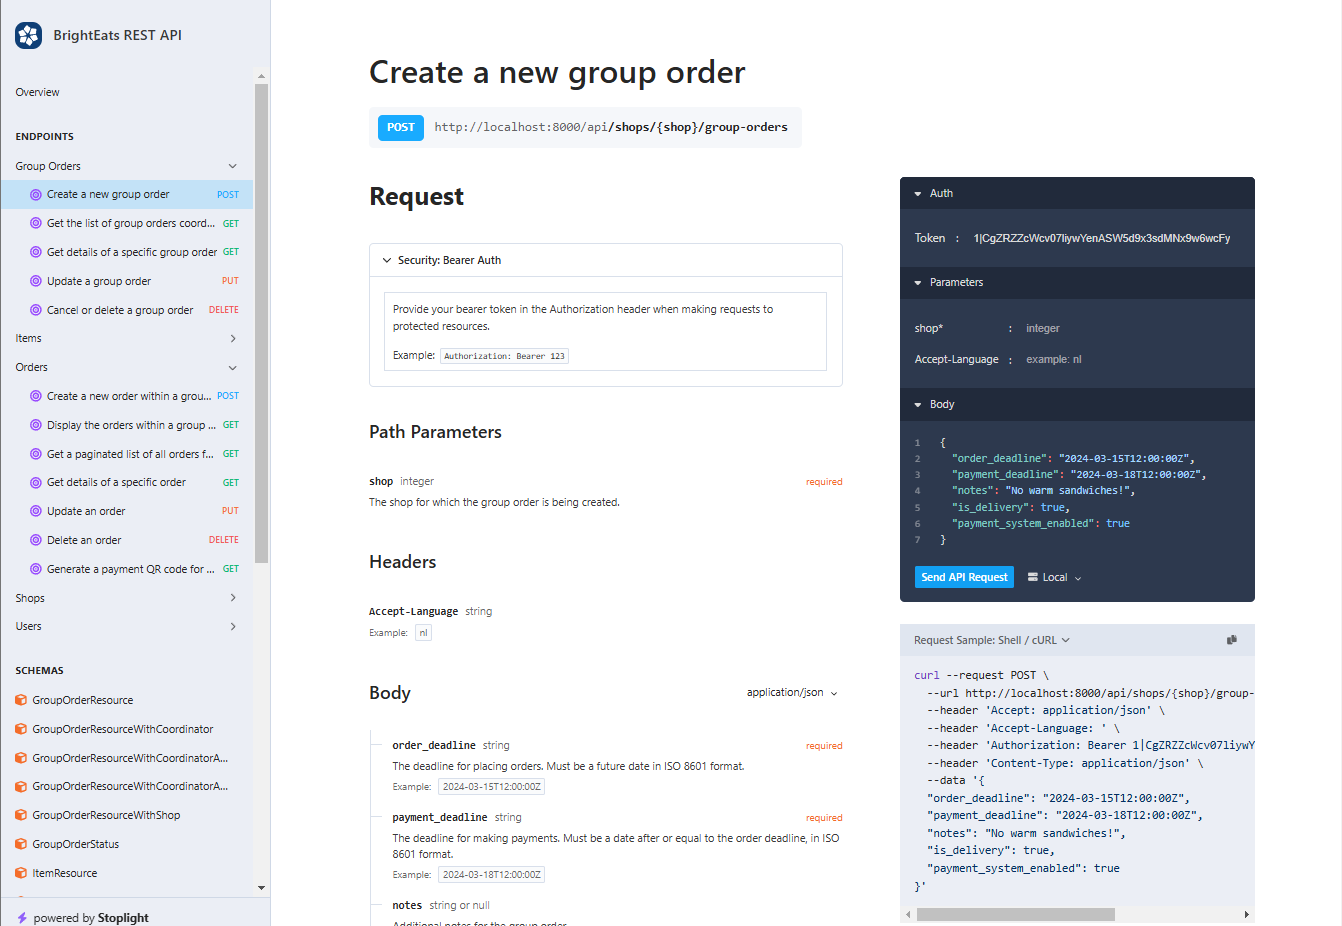
\includegraphics[width=1.0\linewidth]{./graphics/scramble.png}
  \captionof{figure}{Gegenereerde OpenAPI-documentatie met \texttt{dedoc/scramble}}
\end{center}

\section{Resultaten}

De implementatie van RESTful API design principes, in combinatie met de OpenAPI-specificatie, heeft geleid tot significante verbeteringen in de kwaliteit, consistentie en onderhoudbaarheid van de BrightEats API. De gestructureerde code, de uitgebreide documentatie en de geautomatiseerde tests hebben de tijd die nodig is voor debugging aanzienlijk verminderd en het toevoegen van nieuwe features vereenvoudigd. De keuze om HATEOAS niet te implementeren bleek gerechtvaardigd, aangezien de complexiteit en overhead niet opwogen tegen de beperkte meerwaarde in de context van dit project. Aangezien we automatisch gegenereerde documentatie hebben, is HATEOAS niet nodig om de API te ontdekken. Overigens is het gebruik van HATEOAS in een dedicated frontend applicatie vaak omslachtig. HATEOAS kan wel nuttig zijn als een API publiek beschikbaar is of als er meerdere clients zijn die de API gebruiken. Dit is echter meestal niet het geval bij BrightAnalytics.

\section{Conclusie}

De bevindingen van dit onderzoek tonen aan dat RESTful API design en OpenAPI-specificatie concrete voordelen bieden voor de ontwikkeling en het onderhoud van API's bij BrightAnalytics. De gestructureerde aanpak, het consistente gebruik van HTTP-methoden en -statuscodes, en de automatisch gegenereerde documentatie dragen bij aan een verhoogde kwaliteit, consistentie en onderhoudbaarheid van de API's. HATEOAS is niet altijd noodzakelijk en kan, zoals in het geval van de BrightEats API, leiden tot onnodige complexiteit. BrightAnalytics wordt geadviseerd om RESTful principes en OpenAPI te integreren als standaardonderdeel van hun API-ontwikkelingsproces. Verder onderzoek naar de mogelijkheden van automatische validatie met OpenAPI en het uitvoeren van performancetests wordt aanbevolen om de API's verder te optimaliseren. Toekomstig onderzoek zou zich ook kunnen richten op een langetermijnevaluatie van de impact van RESTful design en OpenAPI op de onderhoudskosten, een vergelijking met alternatieve API-stijlen zoals GraphQL, en een diepere analyse van API beveiliging.

\end{multicols}
\end{document}
